\documentclass{classrep}
\usepackage[utf8]{inputenc}
\usepackage{graphicx}
\usepackage{color}
\usepackage{caption} % opcjonalnie, dla lepszego formatowania

\DeclareUnicodeCharacter{00A0}{~}

\studycycle{Informatyka, studia dzienne, inż I st.}
\coursesemester{IV}

\coursename{Sztuczna inteligencja i systemy ekspertowe}
\courseyear{2024/2025}

\courseteacher{Dr. inż. Krzysztof Lichy}
\coursegroup{wtorek, 12:00}

\author{
  \studentinfo{Mikołaj Pawłoś}{258681} \and
  \studentinfo{Emilia Szczerba}{251643}
}

\title{Zadanie drugie: Poprawa lokalizacji UWB przy pomocy sieci neuronowych}

\begin{document}
\maketitle

\section{Cel}
 {Zaprojektowanie i zaimplementowanie sieci neuronowej,
  która pozwoli na korygowanie błędów uzyskanych z systemu pomiarowego.}


\section{Wprowadzenie}
\paragraph{}
\textbf{Sieć neuronowa} (znana również jako \textit{sztuczna sieć neuronowa},
w skrócie \textbf{NN} lub \textbf{ANN})
to model obliczeniowy inspirowany strukturą i funkcjami biologicznych sieci neuronowych.
Sieć neuronowa składa się z połączonych jednostek lub węzłów, zwanych \textbf{sztucznymi neuronami}, które luźno odwzorowują neurony w mózgu.
\paragraph{}
\textbf{Neurony} są połączone \textbf{krawędziami}, które odwzorowują synapsy w mózgu. Każdy sztuczny neuron odbiera sygnały od połączonych z nim neuronów, przetwarza je, a następnie wysyła sygnał do kolejnych połączonych neuronów.
\paragraph{}
„\textbf{Sygnał}” ma postać liczby rzeczywistej, a wyjście neuronu obliczane jest
za pomocą pewnej nieliniowej funkcji sumy jego wejść, zwanej \textbf{funkcją aktywacji}.
\paragraph{}
Siła sygnału w każdym połączeniu jest określana przez \textbf{wagę}, która jest dostosowywana podczas procesu uczenia.

Zazwyczaj neurony grupowane są w \textbf{warstwy}. Różne warstwy mogą wykonywać różne transformacje danych wejściowych.
Sygnały przepływają od pierwszej warstwy (\textit{warstwa wejściowa}) do ostatniej (\textit{warstwa wyjściowa}),
przechodząc być może przez kilka warstw pośrednich (\textit{warstw ukrytych}).
Sieć nazywa się \textbf{głęboką siecią neuronową}, jeśli zawiera co najmniej dwie warstwy ukryte.

\begin{figure}[h!]
	\centering
	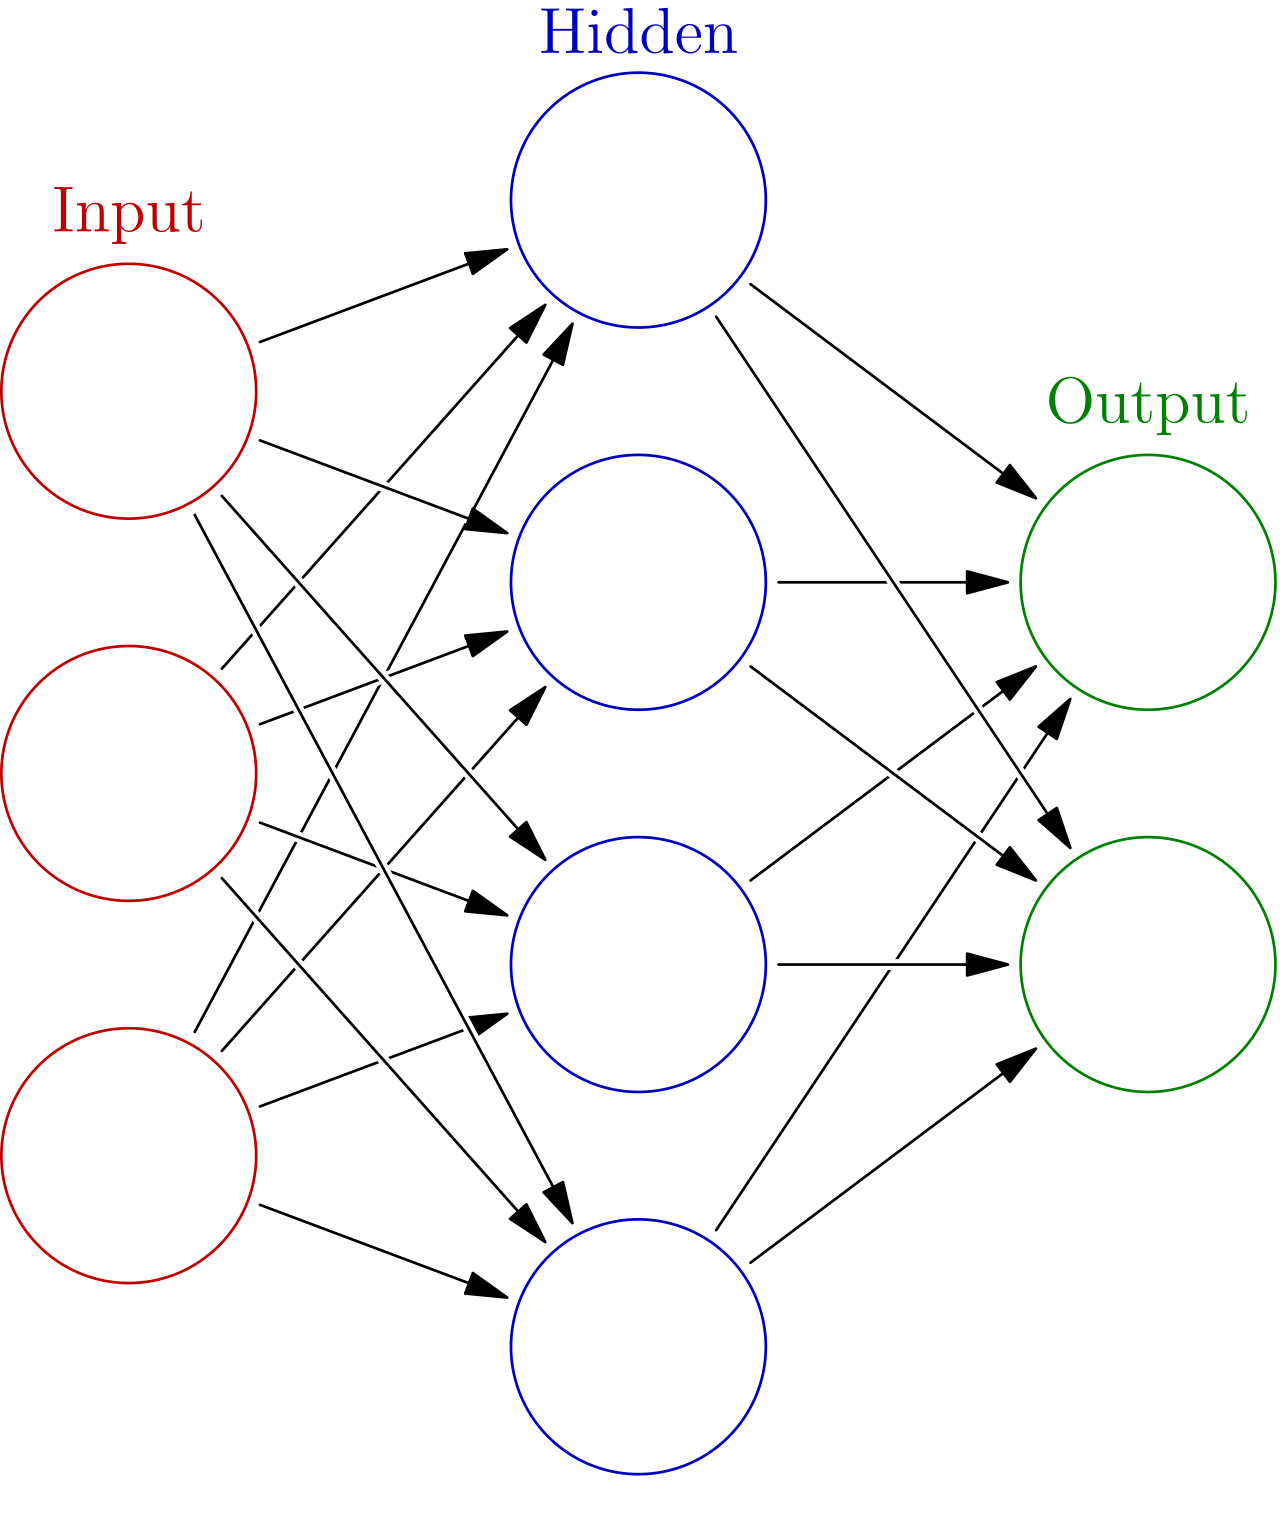
\includegraphics[scale=0.2]{nn.png}
	\caption{Schemat przykładowej sieci neuronowej}
	\label{fig:nn}
\end{figure}

Sztuczne sieci neuronowe są wykorzystywane w różnych zadaniach, takich jak \textit{modelowanie predykcyjne}, \textit{sterowanie adaptacyjne} czy \textit{rozwiązywanie problemów z zakresu sztucznej inteligencji}. Potrafią uczyć się na podstawie doświadczenia i wyciągać wnioski z złożonych i pozornie niepowiązanych danych.

\section{Opis implementacji}
 {\color{blue}
  Należy tu zamieścić krótki i zwięzły opis zaprojektowanych klas oraz powiązań
  między nimi. Powinien się tu również znaleźć diagram UML (diagram klas)
  prezentujący najistotniejsze elementy stworzonej aplikacji. Należy także podać,
  w jakim języku programowania została stworzona aplikacja.}

\section{Materiały i metody}
 {\color{blue}
  W tym miejscu należy opisać, jak przeprowadzone zostały wszystkie badania,
  których wyniki i dyskusja zamieszczane są w dalszych sekcjach. Opis ten
  powinien być na tyle dokładny, aby osoba czytająca go potrafiła wszystkie
  przeprowadzone badania samodzielnie powtórzyć w celu zweryfikowania ich
  poprawności. Przy opisie należy odwoływać się i stosować do
  opisanych w sekcji drugiej wzorów i oznaczeń, a także w jasny sposób opisać
  cel konkretnego testu. Najlepiej byłoby wyraźnie wyszczególnić (ponumerować)
  poszczególne eksperymenty tak, aby łatwo było się do nich odwoływać dalej.}

\section{Wyniki}
 {\color{blue}
  W tej sekcji należy zaprezentować, dla każdego przeprowadzonego eksperymentu,
  kompletny zestaw wyników w postaci tabel, wykresów (preferowane) itp. Powinny
  być one tak ponazywane, aby było wiadomo, do czego się odnoszą. Wszystkie
  tabele i wykresy należy oczywiście opisać (opisać co jest na osiach, w
  kolumnach itd.) stosując się do przyjętych wcześniej oznaczeń. Nie należy tu
  komentować i interpretować wyników, gdyż miejsce na to jest w kolejnej sekcji.
  Tu również dobrze jest wprowadzić oznaczenia (tabel, wykresów), aby móc się do
  nich odwoływać poniżej.}

\section{Dyskusja}
 {\color{blue}
  Sekcja ta powinna zawierać dokładną interpretację uzyskanych wyników
  eksperymentów wraz ze szczegółowymi wnioskami z nich płynącymi. Najcenniejsze
  są, rzecz jasna, wnioski o charakterze uniwersalnym, które mogą być istotne
  przy innych, podobnych zadaniach. Należy również omówić i wyjaśnić wszystkie
  napotkane problemy (jeśli takie były). Każdy wniosek powinien mieć poparcie we
  wcześniej przeprowadzonych eksperymentach (odwołania do konkretnych wyników).
  Jest to jedna z najważniejszych sekcji tego sprawozdania, gdyż prezentuje
  poziom zrozumienia badanego problemu.}

\section{Wnioski}
 {\color{blue}
  W tej, przedostatniej, sekcji należy zamieścić podsumowanie najważniejszych
  wniosków z sekcji poprzedniej. Najlepiej jest je po prostu wypunktować. Znów,
  tak jak poprzednio, najistotniejsze są wnioski o charakterze uniwersalnym.}

\begin{thebibliography}{0}
	\bibitem{l2short} Wikipedia contributors. "Neural network (machine learning)."
	Wikipedia, The Free Encyclopedia. Wikipedia, The Free Encyclopedia,
	29 May. 2025. Web. 29 May. 2025. \end{thebibliography}

{\color{blue}
Na końcu należy obowiązkowo podać cytowaną w sprawozdaniu literaturę, z której
grupa korzystała w trakcie prac nad zadaniem.}

\end{document}
